\section{Experiments}
\label{sec:experiments}

In this section, we evaluate \Endd via minimization of Reverse KL-divergence between the model and a Proxy Dirichlet target. We apply distribution distillation to ensembles of convolutional networks trained on the ImageNet dataset and to ensemble of Transformer models trained on WMT'17 En-De. Our goal here is to demonstrate that given an ensemble, we can successfully distribution-distill it into a single model. Note that we do not provide results for \Endd accomplished by optimizing Dirichlet NLL or forward KL-divergence, because we could not get them to even begin to converge on the tasks considered here. 

\subsection{Setup}
\label{sec:experiments_setup}
We consider two large-scale tasks involving classification: 1000-class image classification and sequence-to-sequence modeling of natural language. For each task, we first train the ensemble of regular models and then distill it with \Endd. For comparison, we also report the average single-model performance along with the following baselines:

\begin{itemize}
\item \textbf{Ensemble} refers to the performance of an ensemble of independently trained models, which was previously shown to yield high quality uncertainty estimates~\cite{deepensemble2017} and to outperform more sophisticated methods using only a few models~\cite{ashukha2020pitfalls}.
\item \textbf{Ensemble Distillation} (EnD) is a common approach to model and ensemble distillation, first proposed in~\cite{hinton2015distilling}. It involves training the student model with the soft target distribution of averaged ensemble predictions. Notably, we do not add the cross-entropy loss for ground truth labels, because we focus on the comparison of distillation objectives and not only classification performance.
\end{itemize}

% TODO discuss why not MC-dropout?
We do not use Hydra~\cite{hydra} or similar multi-head approaches for distilling each separate ensemble member, because with a high number of models in the ensemble and even 1000 classes the computation overhead is no longer negligible. In all experiments with \Endd, we add 1 both to the predicted parameters of the Dirichlet distribution and the Dirichlet proxy parameters.
% : we evaluate the performance of versions without these modifications in Section~\ref{sec:experiments_ablation}

Both for error rejection and out-of-distribution detection, we use several information-theoretic measures uncertainty; in particular, we use entropy of the expected predictive distribution (EoE) for total uncertainty and Reverse Mutual Information (RMI) for knowledge uncertainty throughout this section.
Derivations of these measures both for \Endd and ensembles are available in~\cite{malinin-thesis} and~\cite{malinin-structured-2020}.
For Single and EnD single-model baselines, we use
entropy of the output distribution as the only valid uncertainty estimate.
% the same measures of uncertainty by interpreting exponents of logits as parameters of a Dirichlet distribution. 
% As we show later, in some setups the performance of such models can be surprisingly competitive with that of \Endd and even ensembles; we leave the study of this phenomenon to future work.

\subsection{Large-scale image classification}
\label{experiments:imagenet}

For the first experiment, we run distillation of the ensemble that contains 10 ResNet-50~\cite{resnet} models trained on the ImageNet~\cite{imagenet} image classification dataset. We use the standard training setup outlined in~\cite{touvron2019FixRes}; specifically, we train for 90 epochs using stochastic gradient descent with momentum of 0.9 and a learning rate of $0.1\times B/256$ (first proposed in~\cite{goyal2018accurate}), where B is the per-device batch size multiplied by the number of GPUs. 
In our experiments, we use a single-GPU batch size of 256 and 8 NVIDIA V100 GPUs. The learning rate is divided by 10 every 30 epochs. For data augmentations, we use a standard combination of random resized crops and horizontal flips implemented in the Albumentations library~\cite{albumentations}.
In all experiments, we found it beneficial to initialize the last batch normalization $\gamma$ in each residual branch to zero, which agrees with previous results~\cite{goyal2018accurate, zhang2018residual, rezero}.

For a thorough evaluation of all methods, we use several different characteristics of performance. First, we measure the in-domain classification accuracy on the original ImageNet validation subset~\cite{imagenet}, which is commonly used for comparison of image classification models. Second, we compare the robustness of all approaches to different domain shifts, also measured by accuracy on datasets corresponding to these shifts. In particular, we use adversarial examples from ImageNet-A~\cite{hendrycks2021nae}, corrupted and perturbed versions of original ImageNet validation data from ImageNet-C~\cite{hendrycks2019robustness}, and artistic renditions from ImageNet-R~\cite{hendrycks2020many}. Next, these domain shift and the original validation dataset are used to compare calibration of models with Expected Calibration Error (ECE).
Finally, we measure the out-of-distribution detection error in terms of Receiver Operating Characteristic area under curve (ROC AUC) on the domain shift datasets together with ImageNet-O~\cite{hendrycks2021nae}.

% \begin{itemize}
% \item In-domain classification accuracy
% \item Robustness is specifically classification accuracy for out-of-domain data
% \item Expected calibration error (ECE)
% \item Out-of-domain detection error: , measured in terms of the area under the ROC AUC curve
% \end{itemize}

% Finally, we also evaluate the out-of-distribution detection error, measured in terms of Receiver Operating Characteristic area under curve (ROC AUC).


We report the results for all metrics in Tables~\ref{tab:imagenet_pred} and~\ref{tab:imagenet_ood} for prediction quality and out-of-distribution detection respectively.
Here, the metrics on ImageNet-C are averaged over all degrees of corruption; in Figure~\ref{fig:imagenet_breakdown}, we provide the detailed results of evaluation on each degree separately.
For out-of-distribution detection, we also provide the results of the Dirichlet Proxy to verify that this approximation of the ensemble predictive distribution does not significantly affect its performance.

Table~\ref{tab:imagenet_pred} shows that \Endd is capable of accurate emulation of the ensemble in terms of classification performance: in terms of accuracy, the method displays results on par or slightly better than regular distillation while also having smaller calibration errors. Also, in Table~\ref{tab:imagenet_ood}, it can be seen that for most datasets (except the hardest ImageNet-O) Proxy-Dirichlet distillation can closely match the out-of-distribution performance of the ensemble. As expected, both distillation methods outperform training a single model from scratch while having the same computational complexity.

Furthermore, Figure~\ref{fig:imagenet_breakdown} shows that as the domain shift increases, all models suffer from a drop in accuracy and calibration quality; notably, EnD and \Endd have the same calibration performance on original data, but Dirichlet network distillation has lower calibration errors for the highest degrees of corruption. Unsurprisingly, the further the data is from the original training images, the better the models are at out-of-distribution detection.

\begin{table}
\centering
\small
\caption{Prediction quality results for image classification.}
\label{tab:imagenet_pred}
\begin{tabular}{lcccccccc}
\toprule
{} & \multicolumn{2}{c}{ImageNet-val} & \multicolumn{2}{c}{ImageNet-A} & \multicolumn{2}{c}{ImageNet-C} & \multicolumn{2}{c}{ImageNet-R} \\
{} &          Acc &      ECE &        Acc &       ECE &        Acc &       ECE &        Acc &       ECE \\
\midrule
Single   &     75.9±0.1 &  4.8±0.1 &    4.4±0.2 &  51.1±0.3 &   39.1±0.7 &  11.3±0.7 &   35.0±0.2 &  21.3±0.4 \\
Ensemble &         79.0 &      2.3 &        3.9 &      42.0 &       43.5 &       4.5 &       38.8 &       9.8 \\
EnD      &         77.0 &      1.6 &        3.8 &      46.6 &       40.6 &       5.9 &       36.9 &      16.1 \\
\Endd    &         77.1 &      1.6 &        3.9 &      42.8 &       40.6 &       4.5 &       37.0 &      11.8 \\
\bottomrule
\end{tabular}
\end{table}

\begin{table}
\centering
\small
\caption{Out-of-distribution detection results for image classification.}
\label{tab:imagenet_ood}
\begin{tabular}{lcccccccc}
\toprule
{} & \multicolumn{2}{c}{ImageNet-O} & \multicolumn{2}{c}{ImageNet-A} & \multicolumn{2}{c}{ImageNet-C} & \multicolumn{2}{c}{ImageNet-R} \\
{} &        EoE &   RMI &        EoE &   RMI &        EoE &   RMI &        EoE &   RMI \\
\midrule
Single   &   50.7±0.3 &     - &   85.8±0.1 &     - &   79.9±0.4 &     - &   83.0±0.2 &     - \\
Ensemble &       54.6 &  62.7 &       88.8 &  86.7 &       82.0 &  77.5 &       86.1 &  84.1 \\
Proxy    &       54.6 &  62.9 &       88.8 &  86.5 &       82.0 &  77.3 &       86.1 &  84.0 \\
EnD      &       48.4 &     - &       87.2 &     - &       80.8 &     - &       83.9 &     - \\
\Endd    &       52.0 &  53.2 &       86.8 &  84.6 &       80.1 &  76.9 &       83.7 &  81.4 \\
\bottomrule
\end{tabular}
\end{table}

\begin{figure}
    \centering
    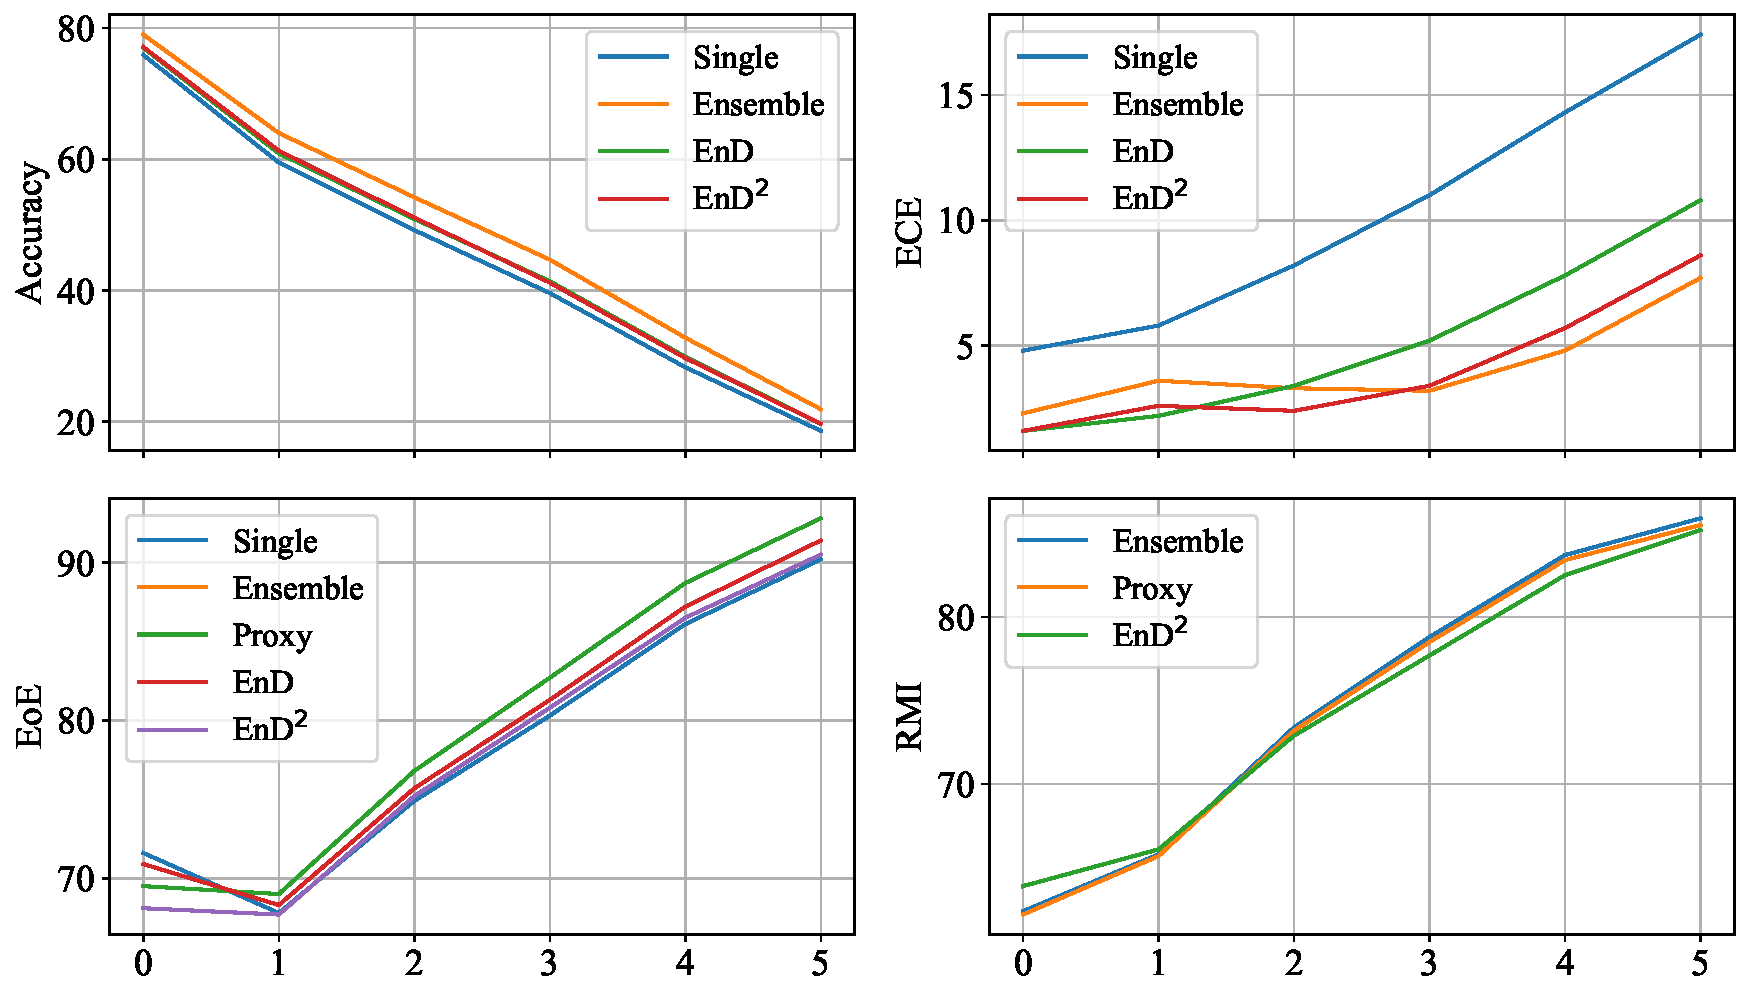
\includegraphics[width=\textwidth]{figures/breakdown.pdf}
    \caption{Performance of image classification models depending on the level of ImageNet-C corruption.  No corruption corresponds to the original ImageNet validation data.}
    \label{fig:imagenet_breakdown}
\end{figure}

\subsection{Machine translation}
\label{experiments:nmt}
For this experiment, we train standard Transformer-big~\cite{vaswani2017attention} models on the WMT'17 English-German machine translation dataset with the vocabulary of 40,000 Byte-Pair Encoding tokens~\cite{sennrich-etal-2016-neural}. Each of the 10 ensemble members is trained with the setup described in~\cite{ott2018scaling}: in particular, we train them for 193,000 steps with Adam~\cite{adam} on 8 NVIDIA V100 GPUs with a batch size of 4096 tokens per GPU. We train all distillation models for 20,000 steps with the increased batch size of 32K tokens. Because our approach requires fitting all 10 ensemble members in GPU memory, we reduce the immediate batch size for each step to 1024, but compensate for it with gradient accumulation over 32 steps. For output generation and estimation of uncertainty measures (where applicable), we use beam search with beam size 5.

To compare the approaches in terms of translation quality, we use the BLEU score~\cite{papineni2002bleu} computed with SacreBLEU~\cite{sacrebleu} and sequence-level Prediction Rejection Ratio~\cite{malinin-thesis} on the newstest14 English-German test set. For out-of-distribution detection, we also compute ROC AUC and use several datasets with different characteristics and degrees of domain shift: sentences with permuted tokens in the input, LibriSpeech~\cite{librispeech} test-clean speech transcriptions, and source sentences from newstest14 in German and French languages respectively. We average the results of both distillation methods over 5 random seeds and provide standard deviations of all metrics.

\begin{table}
\centering
\small
\caption{Prediction quality results for machine translation.}
\label{tab:wmt_pred}
\begin{tabular}{lccc}
\toprule
{} &      BLEU &       EoE &       RMI \\
\midrule
Single   &  28.8±0.1 &  36.0±1.3 &  - \\
Ensemble &      30.1 &      30.2 &      26.0 \\
EnD      &  29.4±0.1 &  35.6±0.4 &  - \\
\Endd    &  29.5±0.1 &  35.9±0.8 &  35.8±0.5 \\
\bottomrule
\end{tabular}
\end{table}

\begin{table}
\centering
\small
\caption{Out-of-distribution detection results for machine translation.}
\label{tab:wmt_ood}
\begin{tabular}{lcccccccc}
\toprule
{} & \multicolumn{2}{c}{Permuted} & \multicolumn{2}{c}{Speech} & \multicolumn{2}{c}{German} & \multicolumn{2}{c}{French} \\
{} &       EoE &       RMI &       EoE &       RMI &       EoE &       RMI &       EoE &       RMI \\
\midrule
Single   &  80.7±1.5 &         - &  73.7±1.2 &         - &  32.8±2.8 &         - &  27.1±6.3 &         - \\
Ensemble &      83.7 &      97.4 &      67.8 &      73.7 &      39.5 &      82.4 &      25.0 &      73.6 \\
EnD      &  79.5±1.1 &         - &  75.9±0.6 &         - &  35.4±1.6 &         - &  15.6±3.2 &         - \\
\Endd    &  78.3±1.6 &  97.1±0.3 &  77.0±0.3 &  78.5±0.2 &  38.3±1.6 &  70.9±0.7 &  15.9±3.0 &  60.1±3.6 \\
\bottomrule
\end{tabular}
\end{table}

Table~\ref{tab:wmt_pred} further confirms the findings made in the previous section: \Endd via Dirichlet-Proxy outperforms regular ensemble distillation in terms of translation quality and sequence-level error detection. Furthermore, in Table~\ref{tab:wmt_ood} we see that, compared to image classification, the OOD performance gap between total uncertainty and knowledge uncertainty is significantly larger. This might be explained by a significantly larger output space (40,000 classes instead of 1000) or the sequential nature of NMT predictions: because the model generates candidates in a large output space of all possible sequences, its prediction entropy might be high regardless of presence of a domain shift.

% \subsection{Ablation study}
% \label{sec:experiments_ablation}


% \begin{table}[t]
% \centering
% \begin{tabular}{@{}lllll@{}}
% \toprule
%  &  & \multicolumn{3}{l}{OOD detection} \\
%  & Accuracy & Imagenet-C & Imagenet-R & Imagenet-A \\ \midrule
% END\textasciicircum{}2 &  &  &  &  \\
% END\textasciicircum{}2+RKL mediator etc &  &  &  &  \\ \midrule
% - target smoothing &  &  &  &  \\
% - shifted parametrization &  &  &  &  \\
% RKL -\textgreater Forward KL &  &  &  &  \\ \bottomrule
% \end{tabular}%
% \end{table}

% Several additional modifications are given in the Appendix\ref{TODOappendix_ablation}